\chapter{Camera Geometry}

In this chapter, we will present all the geometric primitives at the basis of this computer vision treatise, as well as how these will be used to create a camera model that can well express how 3D points are mapped onto the image plane.
In the following chapter, we will then see how this model parameters are estimated. This chapter is based on the second chapter of Szeliski's book~\cite{szeliski}.

\section{Geometric primitives}
In this section, we introduce geometric primitives such as points, lines, planes and their different representations and transformations.
We will consider 2D primitives and then we will analyze their 3D counterparts as well.

\subsection{2D Primitives}

\subsubsection{Points}
A vector $\mathbf{x}=(x,y)\in \mathbb{R}^2$ can also be represented using \keyword{homogeneous coordinates}, i.e.
$$\tilde{\mathbf{x}}=\begin{bmatrix}
\tilde{x} \\
\tilde{y} \\
\tilde{w}
\end{bmatrix}
\in \mathcal{P}^2$$
where $\mathcal{P}^2$ is the 2D \keyword{projective space}, which is built on $\mathbb{R}^3\setminus \mathbf{0}$.

In $\mathcal{P}^2$, every vector $\tilde{\mathbf{x}}$ is identified by an equivalence class s.t. $$\tilde{\mathbf{x}}\mathcal{R}\tilde{\mathbf{x}}' \iff \exists \tilde{w},\tilde{w}\tilde{\mathbf{x}}=\tilde{\mathbf{x}}'.$$

\begin{definition}{Projective space}
    A projective space $\mathcal{P}^{n+1}$ is defined as the quotient set $(\mathbb{R}^n\setminus \mathbf{0}) / \mathcal{R}$.
\end{definition}

To convert back $\tilde{\mathbf{x}}\in \mathcal{P}^2$ into a \keyword{inhomogeneous} vector, it is sufficient to divide all of its components by $\tilde{w}$, obtaining $\bar{\mathbf{x}} = (x, y, 1)$. 

\begin{definition}{}
    $\bar{\mathbf{x}}$ is known as the \textbf{augmented vector} and can be seen as a class representative.
\end{definition}

Though, homogeneous vectors with $\tilde{w}=0$, cannot be retrasformed to inhomogeneous vectors. These points are called \keyword{points at infinity} and are the \q{big deal} of $\mathcal{P}^2$.

\subsubsection{Lines}
A 2D line is usually represented in its explicit form
$$ax+by+c = 0.$$
Defining $\tilde{\mathbf{l}}=(a,b,c)$ and considering the augmented vectors $\bar{\mathbf{x}}$, we can represent the line as
$$\tilde{\mathbf{l}}^{\top}\bar{\mathbf{x}}=0.$$

\begin{observation}{}
$(a,b,1)\in \mathcal{P}^2$ is the normal vector of the line. In fact, taken two random points $\bar{\mathbf{x}}_{1}=(x,y,1)$ and $\bar{\mathbf{x}}_{2}=(x',y',1)$ that lie on the line (hence, $\bar{\mathbf{x}}_{i}^{\top}\tilde{\mathbf{l}}=0, \forall i\in\set{1,2}$), we have
$$a(x - x') + b(y - y') + c - c=0$$ and so $(a,b,1)$ is orthogonal to every vector that lies on the line, since we have made no assumptions on the two points.
\end{observation}

We can divide this equation by the norm of the normal vector $||\mathbf{l}||=\sqrt{a^2 + b^2}$, obtaining
$$\frac{ax + by + c}{\sqrt{a^2 + b^2}}=\hat{n}_{x} x + \hat{n}_{y} y + \overbrace{\frac{c}{\sqrt{a^2 + b^2}}}^{d}=0$$
with $d$ being the distance of the line from the origin and with $\| \mathbf{n} \|=1$.

\begin{observation}{}
    The geometric signed distance from any point $(x_0, y_0)$ to a line defined by $ax + by + c = 0$ is calculated using the standard point-to-line distance formula:
    $$d = \frac{ax_0 + by_0 + c}{\sqrt{a^2 + b^2}}$$
    To find the signed distance specifically from the coordinate origin $(0,0)$ to the line, you substitute $x_0 = 0$ and $y_0 = 0$ into the formula:
    $$d = \frac{c}{\sqrt{a^2 + b^2}}$$
\end{observation}

In a more compact form,
$$\mathbf{l}^{\top} \bar{\mathbf{x}} =
\begin{bmatrix}
\hat{n}_x & \hat{n}_y & d
\end{bmatrix}
\begin{bmatrix}
x \\
y \\
1
\end{bmatrix}
= 0
$$

\begin{observation}{}
    We can express the unit normal vector as $\hat{\mathbf{n}}=(\hat{n}_{x}, \hat{n}_{y})=(\cos \theta, \sin \theta)$ where $\theta$ is the angle between the $x$-axis and $\hat{\mathbf{n}}$. Said $d$ the distance of the line from the origin, we can identify the line by its \textbf{polar coordinates} $(\theta, d)$.
\end{observation}

The line at infinity is the line on which lie all points at infinity. For every point at infinity to lie on it, we must have
$$ax + by + c\cdot0 = 0 \implies ax + by = 0$$
The only way this can happen for all points at infinity is to set $a=b=0$ and any non-null $c$. Since $(0,0,k)\mathcal{R}(0,0,1)$, we set $c=1$ and so the line at infinity is represented by
$$\mathbf{\tilde{l}}^{\top}\tilde{\mathbf{x}} = \begin{bmatrix}
0 & 0 & 1
\end{bmatrix}\begin{bmatrix}
x \\
y \\
w
\end{bmatrix}.$$

Since $\| \hat{\mathbf{n}} \|=0$, normalization is not possible for the line at infinity.

\subsubsection{Duality principle}
By definition, a point $\tilde{\mathbf{x}}$ lies on a line $\tilde{\mathbf{l}}$ if their dot product is null:
$$\tilde{\mathbf{x}}^{\top}\tilde{\mathbf{l}}=0.$$
A point $\tilde{\mathbf{x}}$ that is the intersection of two lines $\tilde{\mathbf{l}}_{1}$, $\tilde{\mathbf{l}}_{2}$ lies on both of them:
$$\begin{cases}
\tilde{\mathbf{x}}^{\top}\tilde{\mathbf{l}}_{1}=0 \\
\tilde{\mathbf{x}}^{\top}\tilde{\mathbf{l}}_{2}=0
\end{cases}$$

Now, recall that two vectors are orthogonal when their dot product is null. So, the intersection of the two lines is orthogonal to both of them.
We can conclude that their intersection $\tilde{\mathbf{x}}$ is given by their cross product
$$\tilde{\mathbf{x}}=\tilde{\mathbf{l}}_{1}\times \tilde{\mathbf{l}}_{2}$$
since every other scaling of $\tilde{\mathbf{x}}$ is equivalent.
Analogously, the line joining two points can be written as
$$\tilde{\mathbf{l}}=\tilde{\mathbf{x}}_{1}\times \tilde{\mathbf{x}}_{2}.$$

This is known as the \keyword{duality principle} between lines and points in projective geometry.

\subsubsection{Conics}
A conic section is a 2D curve formed by the intersection of a flat plane and a 3D cone.

We can express a conic section using a \emph{quadric equation}, which is a compact way of expressing the general second-degree polynomial equation for conics:
$$\tilde{\mathbf{x}}^T \mathbf{Q} \tilde{\mathbf{x}} = Ax^2 + Bxy + Cy^2 + Dx + Ey + F = 0$$
where $\tilde{\mathbf{x}}$ represents a point in homogeneous coordinates and $\mathbf{Q}$ is a symmetric matrix defining the shape.

Depending on the values of the coefficients inside the matrix $\mathbf{Q}$, this equation represents different familiar geometric shapes:
\begin{itemize}
\item \textbf{Circle}. Formed when the intersecting plane is strictly perpendicular to the cone's axis. Its equation is $x^2 + y^2 - r^2 = 0$;
\item \textbf{Ellipse}. Formed when the plane is tilted but still cuts entirely through one half of the cone. Its equation is $\frac{x^2}{a^2} + \frac{y^2}{b^2} - 1 = 0$;
\item \textbf{Parabola}. Formed when the plane is exactly parallel to the slanted side of the cone. Its equation is $y - ax^2 = 0$;
\item \textbf{Hyperbola}. Formed when the steep plane intersects both the upper and lower halves of a double cone. Its equation is $\frac{x^2}{a^2} - \frac{y^2}{b^2} - 1 = 0$
\end{itemize}

Quadric equations play useful roles in the study of multi-view geometry and camera calibration.

\subsection{3D Primitives}

\subsubsection{Points}
Points in $\mathbb{R}^3$ can be embedded in $\mathcal{P}^3$, as we have seen with 2D points.

\subsubsection{Planes}
A 3D plane in the general equation
$$ax+by+cz+d=0$$
can be once again represented with $\bar{\mathbf{x}}^{\top}\tilde{\mathbf{m}}$ with $\bar{\mathbf{x}}$ being the augmented vector and $\tilde{\mathbf{m}}=(a,b,c,d)$. The normal vector of such a 3D plane is $\hat{\mathbf{n}}=(a,b,c)$.

Once again, by dividing $\tilde{\mathbf{m}}$ by $\| \hat{\mathbf{n}} \|$, we obtain an equivalent representation of the plane with unitary normal vector and the distance from the origin as the last component:
$$\mathbf{m}=(\hat{n}_{x},\hat{n}_{y},\hat{n}_{z},d).$$
The only plane that cannot be normalized is the plane at infinity, which is unsurprisingly (at this point) represented by
$$\tilde{\mathbf{m}}=(0,0,0,1).$$
While we represent the normal vector of a line in $\mathcal{P}^2$ in polar coordinates, we use \emph{spherical coordinates} for a plane in $\mathcal{P}^3$:
$$\hat{\mathbf{n}}=\begin{bmatrix}
\cos \theta \cos \phi \\
\sin \theta \cos \phi \\
\sin \theta
\end{bmatrix}$$

\subsubsection{Lines}
A 3D line can be represented by fixing two points that lie on it $\mathbf{p},\mathbf{q}\in \mathbb{R}^3$ and taking their linear combinations:
$$\mathbf{r}=(1-\lambda)\mathbf{p}+\lambda \mathbf{q}.$$
With homogeneous coordinates:
$$\tilde{\mathbf{r}}=\mu \tilde{\mathbf{p}} + \lambda \tilde{\mathbf{q}}.$$

A special case is when $\tilde{\mathbf{q}}$ is at infinity. In this case, we can see $\tilde{\mathbf{q}}=(\hat{d}_{x},\hat{d}_{y},\hat{d}_{z},0)$ as the direction of $\mathbf{r}$ (the 3D line in inhomogeneous coordinates), which we can then express as
$$\mathbf{r}=\mathbf{p}+\lambda\hat{\mathbf{d}}.$$
However, this representation has six \keyword{degrees of freedom} (DOF), while we will see in a moment that we can get an equivalent representation with four.

\begin{definition}{Degrees of freedom (DOF)}
    A \textbf{degree of freedom} (DOF) represents the minimum number of parameters that have to be determined to uniquely identify a transformation within its family (e.g. $n\times n$ matrices).
\end{definition}

In fact, we can constrain our two points to lie on two specific, fixed 3D planes, so that we can consider only the 2D coordinates of the two points (relative to their plane) to represent the 3D line.
However, if the two fixed 3D planes are parallel, we cannot represent a 3D line that lies completely on one of the two planes.

Intuitively, we could also identify a 3D line as the intersection between two 3D planes. However, this representation has eight degree of freedom and is hence inconvenient. Figure shows this graphically.

\begin{figure}[h]
    \centering
    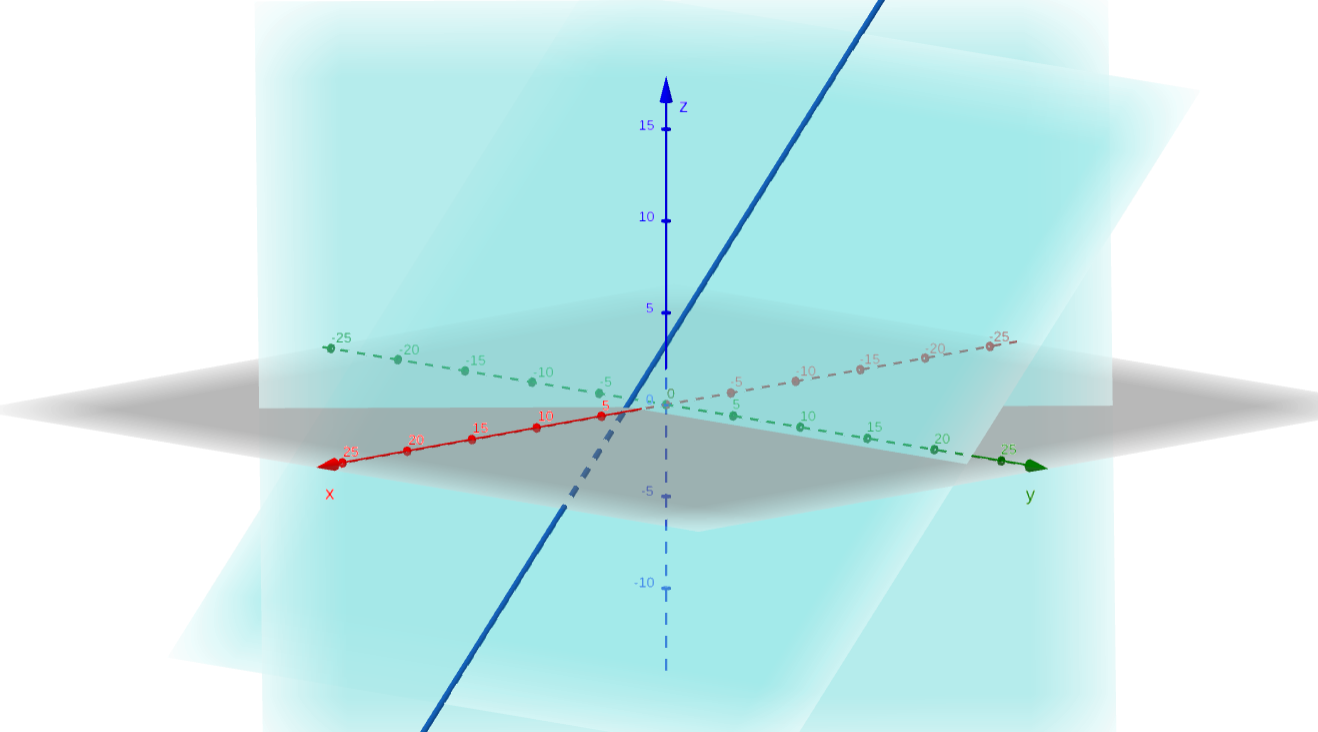
\includegraphics[width=0.5\textwidth]{../_files/_images/planes_intersection.png}
    \caption{In this figure, we can see the 3D generated by the intersection of two planes. This was built with the GeoGebra Calculator, available at \url{https://www.geogebra.org/calculator}.}
    \label{fig:plane-intersection}
\end{figure}

Another more general (and DOF-efficient) way of determining a 3D line is with a skew-symmetric matrix $\mathbf{L}\in \mathbb{R}^{4\times 4}$ in \emph{Plücker coordinates}:
$$\mathbf{L}=\tilde{\mathbf{p}}\tilde{\mathbf{q}}^{\top} + \tilde{\mathbf{q}}\tilde{\mathbf{p}}^{\top}.$$

\begin{definition}{Skew-symmetric matrix}
    $\mathbf{L}$ is a skew-symmetric matrix if and only if $\mathbf{L}^{\top} = -\mathbf{L}$.
    In words, a skew-symmetric matrix has a main diagonal consisting entirely of zeros, and the elements across the diagonal mirror each other with opposite signs.
\end{definition}

The actual Plücker coordinates are the six independent, non-zero entries found within $\mathbf{L}$ (typically taken from the upper-right triangle).
Since $\mathbf{L}$ is always homogeneous, meaning that uniformly scaling its values does not change the underlying line geometry, we remove a DOF.
Moreover, since $\det \mathbf{L}=0$, there is a quadratic relationship between the six coordinates, removing another DOF, resulting in four DOF.

\subsubsection{Quadrics}
The 3D analog of a conic section is a quadric surface, which can be represented in the very same format of 2D conics:
$$\bar{\mathbf{x}}^T \mathbf{Q} \bar{\mathbf{x}} = 0.$$

\section{Transformations}
Having defined the geometric primitives, we can now turn our attention to how they can be transformed.
For each of the below presented tranformations, we will describe their DOF and which geometric property it preserves at least.
We consider the following hierarchy (on the right the weaker property): orientation $\succ$ lengths $\succ$ angles $\succ$ parallel lines $\succ$ vertical lines.
This means that a transformation that preserves (say) angles, also preserves parallel lines and vertical lines.

\subsection{2D Transformations}

\subsubsection{Translation}
Considering homogeneous coordinates, translation can be represented with the following multiplication:
$$\bar{\mathbf{x}}'=\begin{bmatrix}
\mathbf{I}_{2\times 2} & \mathbf{t} \\
\mathbf{0}^{\top} & 1
\end{bmatrix} \bar{\mathbf{x}}.$$
Translation has 2 DOF: one for the $x$ and one for the $y$ coordinate. A translation preserves orientation.

\subsubsection{Rigid body motion}
A 2D rigid body motion (i.e. a translation + rotation) can be written as
$$\bar{\mathbf{x}}'=\begin{bmatrix}
\mathbf{R} & \mathbf{t} \\
\mathbf{0}^{\top} & 1
\end{bmatrix} \bar{\mathbf{x}}$$
where $\mathbf{R}=\begin{bmatrix}\cos \theta & -\sin \theta \\ \sin \theta & \cos \theta\end{bmatrix}$.
Rigid body motion has $3$ DOF: two for the translation, one for the rotation. This transformation preserves lengths.

\subsubsection{Scaled rotation}
A scaled rotation is fundamentally a rigid body motion that can scale the $x$ and $y$ coordinates independently:
$$\bar{\mathbf{x}}'=\begin{bmatrix}
a & -b & t_{x} \\
b & a & t_{y} \\
0 & 0 & 1
\end{bmatrix}\bar{\mathbf{x}}.$$
It has $4$ DOF and preserves angles.

\subsubsection{Affine}
An affine transformation is defined as:
$$\bar{\mathbf{x}}'=\begin{bmatrix}
a_{11} & a_{12} & a_{13} \\
a_{21} & a_{22} & a_{23} \\
0 & 0 & 1
\end{bmatrix}\bar{\mathbf{x}}.$$
It has $6$ DOF and preserves parallel lines.

\subsubsection{Projective}
Also known as \keyword{homography}, a projective transformation can be represented as:$$\bar{\mathbf{x}}'=\tilde{\mathbf{H}}\bar{\mathbf{x}}$$
where $\tilde{\mathbf{H}}\in \mathbb{R}^3$ is homogeneous, i.e. $\tilde{\mathbf{H}}\equiv k\tilde{\mathbf{H}}$.
A projective transform has $8$ DOF ($9$ DOF minus a scale factor) and preserves vertical lines.

Projective transformations are the only that can map points not at infinity to points at infinity and vice versa.

\paragraph{Co-vectors}
So far, we have described how a homography transforms points, but what about lines?

Applying the substitution $\tilde{\mathbf{x}}'=\tilde{\mathbf{H}}\tilde{\mathbf{x}}$, we obtain
$$\tilde{\mathbf{l}}'^{\top}\tilde{\mathbf{x}}'=\tilde{\mathbf{l}}'^{\top}\tilde{\mathbf{H}}\tilde{\mathbf{x}}=(\tilde{\mathbf{H}}^{\top}\tilde{\mathbf{l}}')^{\top}\tilde{\mathbf{x}}=\tilde{\mathbf{l}}^{\top}\tilde{\mathbf{x}}=0.$$

\begin{note}{}
    Since $(\mathbf{AB})^{\top}=\mathbf{B}^{\top}\mathbf{A}^{\top}$, we can write:
    $$(\tilde{\mathbf{H}}^{\top}\tilde{\mathbf{l}}')^{\top}=\tilde{\mathbf{l}}'^{\top}(\tilde{\mathbf{H}}^{\top})^{\top}=\tilde{\mathbf{l}}'^{\top}\tilde{\mathbf{H}}$$
\end{note}

Since $(\tilde{\mathbf{H}}^{\top}\tilde{\mathbf{l}}')=\tilde{\mathbf{l}}$, we conclude that $\tilde{\mathbf{l}}'=\tilde{\mathbf{H}}^{-\top}\tilde{\mathbf{l}}$ and so the projective transformation applies differently between points and lines, that are said \emph{co-vectors}.

\begin{definition}{Co-vector}
    A \textbf{co-vector} is a geometric entity, such as a 2D line or a 3D normal vector, that transforms differently than standard points when a space undergoes a projective transformation.
\end{definition}

Since $\tilde{\mathbf{H}}$ is homogeneous, $\tilde{\mathbf{H}}^{-\top}$ is equivalent to the adjoint of $\tilde{\mathbf{H}}$.

\begin{definition}{Adjoint matrix}
An \textbf{adjoint matrix} (specifically the classical adjoint or adjugate matrix in linear algebra) is formed by taking the transpose of a matrix's cofactor matrix. Its fundamental mathematical property is that it is proportional to the exact inverse of the matrix, defined by the relationship $\mathbf{H}^{-1} = \frac{\text{adj}(\mathbf{H})}{\det(\mathbf{H})}$.
\end{definition}

\begin{definition}{Cofactor matrix}
A cofactor matrix is a square matrix of the exact same dimensions as the original, where every individual element has been replaced by its corresponding mathematical \textbf{cofactor}.

To calculate the cofactor for a specific element located at row $i$ and column $j$ ($a_{ij}$), you perform two steps:

\begin{enumerate}
\item Calculate the Minor ($M_{ij}$): Delete the entire $i$-th row and $j$-th column from the original matrix. Calculate the determinant of the smaller matrix that remains.
\item Apply the Sign Alternation: Multiply that minor by $(-1)^{i+j}$. This mathematically applies a standard \q{checkerboard} pattern of alternating positive and negative signs across the grid of the matrix.
\end{enumerate}

The formula for a single cofactor $C_{ij}$ is:
$$C_{ij} = (-1)^{i+j} M_{ij}$$
The complete cofactor matrix is built by repeating this calculation for every single position in the original matrix. Taking the transpose of this final grid of cofactors is what produces the adjoint matrix.

Every element in a cofactor matrix is fundamentally a computed fragment of the original matrix's determinant. If you take the dot product of any row in a square matrix $A$ with the exact corresponding row in its cofactor matrix $C$, the result is always the determinant of $A$:
$$a_{i1}C_{i1} + a_{i2}C_{i2} + \dots + a_{in}C_{in} = \det(A)$$
Conversely, if you multiply a row of $A$ by the cofactors of a *different* row, the result is mathematically forced to be exactly zero. This orthogonal relationship is why multiplying a matrix by the transpose of its cofactor matrix (the adjoint) perfectly yields the identity matrix scaled by the determinant: $A \cdot \text{adj}(A) = \det(A)I$.
\end{definition}

\subsubsection{Stretch}
The stretch transformation applies independent scaling and translation to the $x$ and $y$ coordinates:
$$\mathbf{x}'=\begin{bmatrix}
s_{x} & 0 & t_{x} \\
0 & s_{y} & t_{y}
\end{bmatrix} \bar{\mathbf{x}}$$
where $\bar{\mathbf{x}}$ is the augmented vector.

\subsection{3D Transformations}

\subsubsection{Translation}
A 3D translation can be represented as
$$\bar{\mathbf{x}}'=\begin{bmatrix}
\mathbf{I}_{3 \times 3} & \mathbf{t} \\
\mathbf{0}^{\top} & 1
\end{bmatrix} \bar{\mathbf{x}}.$$
It has 3 DOF: one for each translation component.

\subsubsection{Affine}
A 3D affine transformation can be represented as
$$\bar{\mathbf{x}}'=\begin{bmatrix}
a_{11} & a_{12} & a_{13} & a_{14} \\
a_{21} & a_{22} & a_{23} & a_{24} \\
0 & 0 & 0 & 1
\end{bmatrix}\bar{\mathbf{x}}$$
with $\mathbf{A}$ being a $4\times4$ matrix. This transformation has $8$ DOF.

\subsubsection{Rotations}
In general, 3D rotations can be expressed as
$$\bar{\mathbf{x}}'=\begin{bmatrix}
\mathbf{R} & \mathbf{0} \\
\mathbf{0}^{\top} & 1
\end{bmatrix}\bar{\mathbf{x}}$$
with $\mathbf{R}$ being a $3\times 3$ orthonormal rotation matrix s.t. $\mathbf{R}\mathbf{R}^{\top}=\mathbf{I}_{3 \times 3}$ and $\det\mathbf{R}=1$.

Describing the $\mathbf{R}$ matrix is not as straightforward as in the 2D case, since several ways are possible.

\paragraph{Euler angles}
A rotation matrix can be formed as the product of three separate $3 \times 3$ transformation matrices (one for each cardinal axis).

In this model, each primary axis has a standard rotation matrix for a given angle ($\alpha$, $\beta$, or $\gamma$), assuming a right-handed coordinate system (index finger points in the X-axis positive direction, middle finger in Y-axis positive direction, thumb in Z-axis positive direction):
\begin{itemize}
\item Rotation around the X-axis (Roll):
    $$R_x(\alpha) = \begin{bmatrix} 1 & 0 & 0 \\ 0 & \cos\alpha & -\sin\alpha \\ 0 & \sin\alpha & \cos\alpha \end{bmatrix}$$

\item Rotation around the Y-axis (Pitch):
    $$R_y(\beta) = \begin{bmatrix} \cos\beta & 0 & \sin\beta \\ 0 & 1 & 0 \\ -\sin\beta & 0 & \cos\beta \end{bmatrix}$$

\item Rotation around the Z-axis (Yaw):
    $$R_z(\gamma) = \begin{bmatrix} \cos\gamma & -\sin\gamma & 0 \\ \sin\gamma & \cos\gamma & 0 \\ 0 & 0 & 1 \end{bmatrix}$$
\end{itemize}

The final 3D rotation matrix $\mathbf{R}$ is the product of these three matrices. Because matrix multiplication is non-commutative ($A \times B \neq B \times A$), the order in which you apply the matrices fundamentally changes the final rotation.

A common sequence in aerospace and computer graphics is the Z-Y-X sequence.
If you are applying the rotation to a column vector $v$, the transformations are applied right-to-left:
$$R = R_z(\gamma) R_y(\beta) R_x(\alpha)$$
$$v' = R \cdot v$$
This means the object is first rotated around X, then the resulting object is rotated around Y, and finally around Z.

However, Euler angles suffer from \emph{Gimbal lock}: if the middle rotation (e.g., the Y-axis pitch) aligns the first and third axes (e.g., pitching exactly 90 degrees straight up), the system loses a degree of freedom.
Rotations around the X and Z axes will now produce the exact same motion, making smooth interpolation impossible.\footnote{You can watch a nice, animated explanation of Euler angles and gimbal lock at this link: \url{https://www.youtube.com/watch?v=BczeMqU_u2Y}.}

Moreover, Gimbal lock results in angle dramatic changes in response to a tiny change in rotation, making this rotation model not usable in ML techniques as it would be impossible to move smoothly in the parameter space.

\paragraph{Axis/angle}
Any 3D rotation can be described as a single rotation by an angle $\theta$ around a fixed axis defined by a unit vector $\hat{\mathbf{n}}$.
Combining these into a single vector $\mathbf{\omega} = \theta \hat{\mathbf{n}}$ (an axis-angle representation) compactly encodes both the direction of the rotation axis (via the vector's direction) and the magnitude of the rotation (via the vector's length). 

Let's see how to apply a rotation around $\hat{\mathbf{n}}$ with angle $\theta$ to a 3D vector $\mathbf{v}$.
We will refer to the rotated vector as $\mathbf{u}$.
First, note that $\mathbf{v}_{\parallel}$, the $\mathbf{v}$ component that is parallel to $\hat{\mathbf{n}}$, will not be affected by the rotation.
This component is calculated as:
$$\mathbf{v}_{\parallel}=\hat{\mathbf{n}}(\hat{\mathbf{n}}^{\top}\mathbf{v} )=(\hat{\mathbf{n}}\hat{\mathbf{n}}^{\top})\mathbf{v}.$$

Geometrically, we can see the dot product $\mathbf{a}^{\top}\mathbf{b}$ as the length of the projection of $\mathbf{a}$ onto $\mathbf{b}$, scaled by $||\mathbf{b}||$.
Vice versa, we can also see the same product as the length of the projection of $\mathbf{b}$ onto $\mathbf{a}$, scaled by $||\mathbf{a}||$.

Since $\| \hat{\mathbf{n}} \| =1$, the dot product $\hat{\mathbf{n}}^{\top}\mathbf{v}$ is exactly the projection length.
So, multiplying this quantity by $\hat{\mathbf{n}}$ yields the projection vector of $\mathbf{v}$ onto $\hat{\mathbf{n}}$.

The affected component is the orthogonal one:
$$\mathbf{v}_{\perp}=\mathbf{v}-\mathbf{v}_{\parallel}=(\mathbf{I}-\hat{\mathbf{n}}\hat{\mathbf{n}}^{\top})\mathbf{v}.$$
This vector is orthogonal to $\hat{\mathbf{n}}$ and we can rotate it by $90$ degrees by computing its cross product with $\hat{\mathbf{n}}$:
$$\mathbf{v}_{\times}=\hat{\mathbf{n}}\times \mathbf{v}_{\perp}.$$
Another way of expressing this cross product is with a skew-symmetric matrix:
$$\mathbf{v}_{\times}=\hat{\mathbf{n}}\times \mathbf{v}_{\perp}=[\hat{\mathbf{n}}]_{\times}\mathbf{v}=\begin{bmatrix}
0 & -\hat{n}_{z} & \hat{n}_{y} \\
\hat{n}_{z} & 0 & -\hat{n}_{x} \\
-\hat{n}_{y} & \hat{n}_{x} & 0
\end{bmatrix}\mathbf{v}$$

By rotating this last one by another $90$ degrees, we obtain $-\mathbf{v}_{\perp}$:
$$\mathbf{v}_{\times \times}=[\hat{\mathbf{n}}]_{\times}\mathbf{v}_{\times}=[\hat{\mathbf{n}}]_{\times}^2 \mathbf{v}=-\mathbf{v}_{\perp}.$$
Now, we can see $\mathbf{v}_{\parallel}$ as:
$$\mathbf{v}_{\parallel}=\mathbf{v}-\mathbf{v}_{\perp}=\mathbf{v}+\mathbf{v}_{\times \times}=(\mathbf{I}+[\hat{\mathbf{n}}]_{\times}^2)\mathbf{v}.$$
We know that $\mathbf{u}_{\parallel}=\mathbf{v}_{\parallel}$ (the parallel $\mathbf{v}$ component does not change). We must only determine $\mathbf{u}_{\perp}$. 
At this point, we build a 2D plane with primary axis $\mathbf{v}_{\perp}$ and secondary axis $\mathbf{v}_{\times}$ so that we can express $\mathbf{u}_{\perp}$ as:
$$\begin{aligned}
\mathbf{u}_{\perp}&=\cos \theta \mathbf{v}_{\perp} + \sin \theta \mathbf{v}_{\parallel} \\
&=\cos \theta(-[\hat{\mathbf{n}}]_{\times}^2\mathbf{v}) + \sin \theta([\hat{\mathbf{n}}]_{\times}\mathbf{v}) \\
&=([\hat{\mathbf{n}}]_{\times}\sin \theta - [\hat{\mathbf{n}}]_{\times}^2\cos \theta)\mathbf{v}
\end{aligned}$$

\begin{figure}[h]
    \centering
    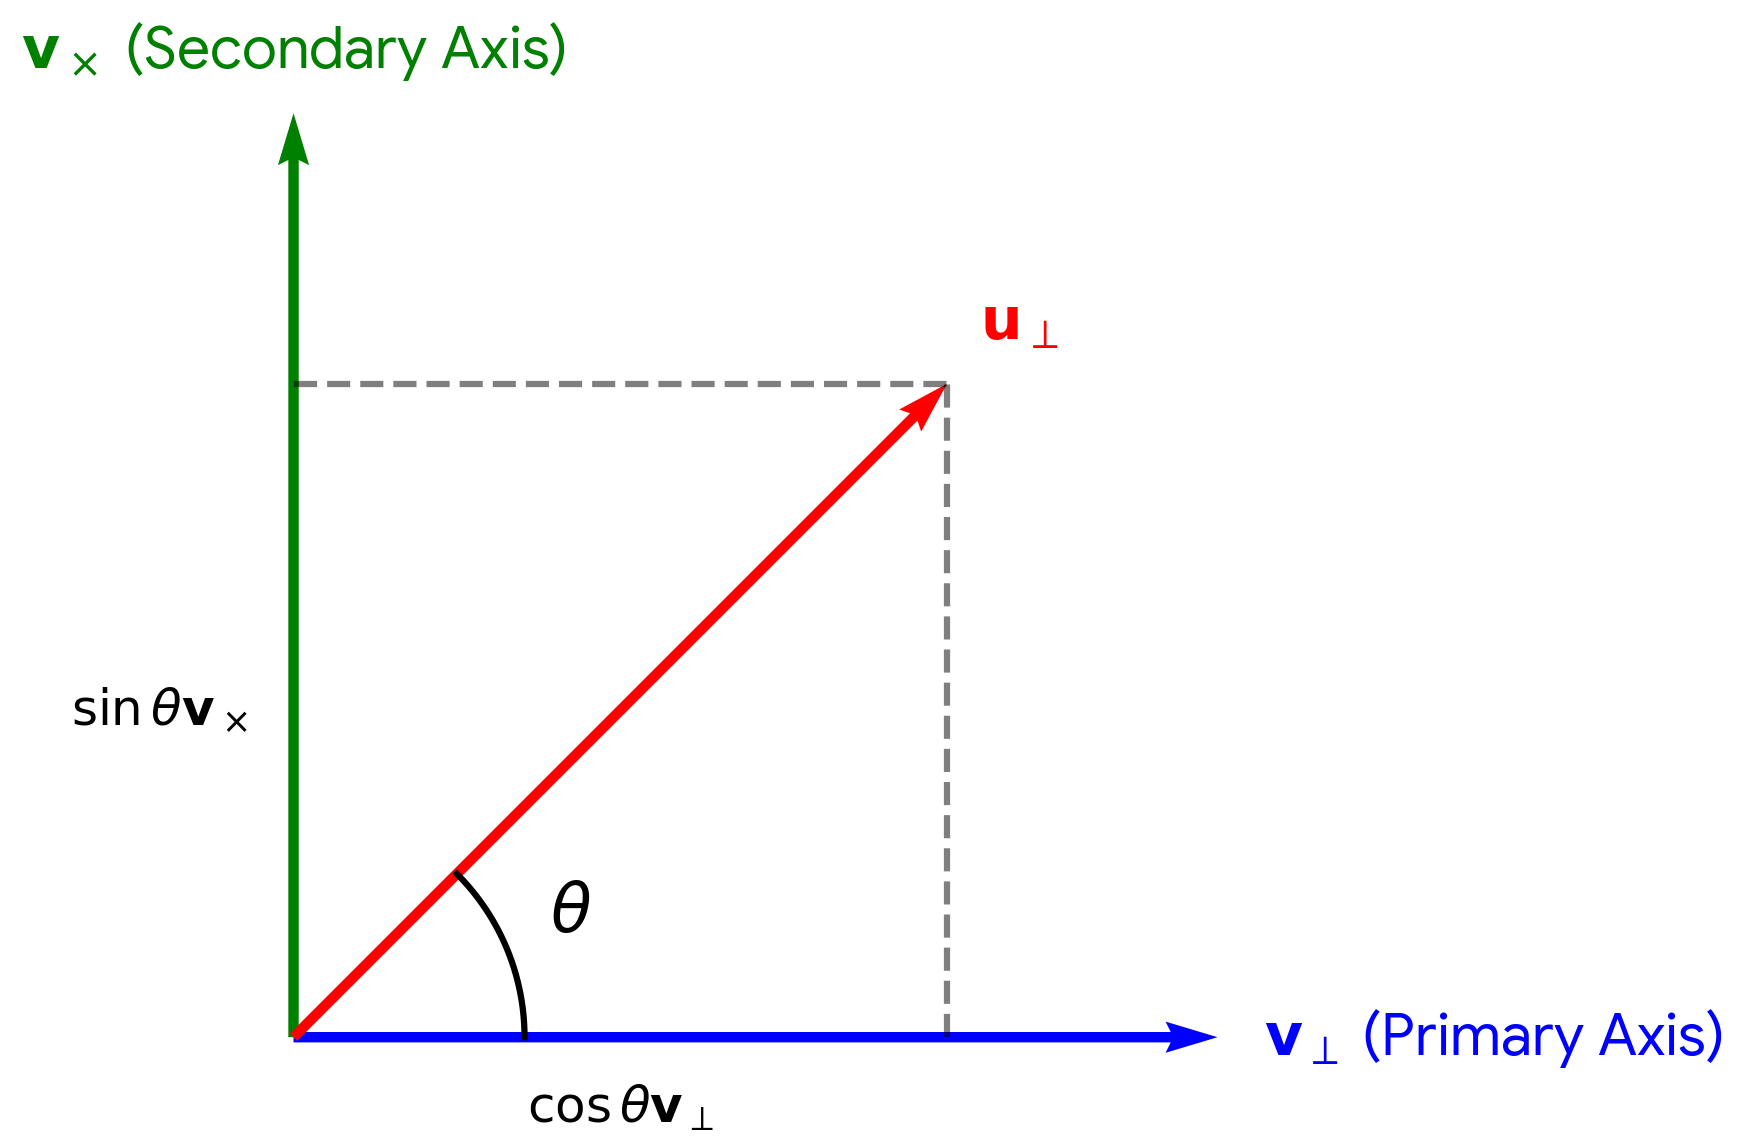
\includegraphics[width=0.5\textwidth]{../_files/_images/local_reference_system.png}
    \caption{The new local reference system. You can see where $\mathbf{u}_{\perp}$ arises from.}
    \label{fig:local-reference-system}
\end{figure}

We can now calculate $\mathbf{u}$ as:
$$\begin{aligned}
\mathbf{u}&=\mathbf{u}_{\parallel}+\mathbf{u}_{\perp} \\
&=\mathbf{v}_{\parallel}+\mathbf{u}_{\perp} \\
&=(\mathbf{I}+[\hat{\mathbf{n}}]_{\times}^2)\mathbf{v}+([\hat{\mathbf{n}}]_{\times}\sin \theta - [\hat{\mathbf{n}}]_{\times}^2\cos \theta)\mathbf{v} \\
&= (\mathbf{I} + [\hat{\mathbf{n}}]_{\times}\sin \theta + (1-\cos \theta)[\hat{\mathbf{n}}]_{\times}^2)\mathbf{v}.
\end{aligned}$$
Finally, we are now able to express a 3D rotation as a function of an axis and an angle:
$$\mathbf{u}=\mathbf{R}(\hat{\mathbf{n}},\theta)\cdot\mathbf{v}$$
where $\mathbf{R}(\hat{\mathbf{n}},\theta)=(\mathbf{I} + [\hat{\mathbf{n}}]_{\times}\sin \theta + (1-\cos \theta)[\hat{\mathbf{n}}]_{\times}^2)\mathbf{v}$, which is known as \emph{Rodrigues' formula}.

When $\theta$ (expressed in radians) is small, Rodrigues's formula can be approximated to
$$\mathbf{R}(\hat{\mathbf{n}}, \theta)\approx \mathbf{I}+[\hat{\mathbf{n}}]_{\times}\theta$$
which makes $\mathbf{R}$ depend linearly on $\hat{\mathbf{n}}$, $\theta$. 

\paragraph{Quaternions}
Quaternions were formulated by Hamilton as an extension of complex numbers, defined as $q = w + x\mathbf{i} + y\mathbf{j} + z\mathbf{k}$, with $\mathbf{i},\mathbf{j},\mathbf{k}$ being the basis vectors for the 3D part of quaternions.
A 3D vector can be embedded into this space as a \q{pure} quaternion with $w=0$.

A \keyword{unit quaternion} is a unit length 4-vector that can be written as $$\mathbf{q}=(x,y,z,w)=(\mathbf{v},w).$$with $\| \mathbf{q} \|=1$. So, unit quaternions live on the unit sphere.

Differently from the axis/angle representation, unit quaternions offer a way to uniquely represent a 3D rotation (actually $\mathbf{q}$ and $-\mathbf{q}$ represent the same rotation).

\paragraph{Rotation axis}
We express our rotation axis as
$$\hat{\mathbf{n}}=\hat{n}_{x}\mathbf{i} + \hat{n}_{y}\mathbf{j} + \hat{n}_{z}\mathbf{k}$$
which can be seen as an imaginary unit for quaternions. In fact,
$$
\hat{n}\hat{n} = n_x^2\mathbf{i}^2 + n_y^2\mathbf{j}^2 + n_z^2\mathbf{k}^2 + n_x n_y(\mathbf{ij} + \mathbf{ji}) + n_y n_z(\mathbf{jk} + \mathbf{kj}) + n_z n_x(\mathbf{ki} + \mathbf{ik}) \\
$$
but the cross-terms cancel out (imaginary units anti-commute):
$$\begin{aligned}
\hat{n}\hat{n} &= n_x^2\mathbf{i}^2 + n_y^2\mathbf{j}^2 + n_z^2\mathbf{k}^2 \\
&=n_x^2(-1) + n_y^2(-1) + n_z^2(-1) \\
&=-(n_x^2 + n_y^2 + n_z^2) = -1 
\end{aligned}$$
So, the quaternion product between $\hat{n}$ and itself is $-1$. Note that the dot product $\hat{n}\cdot\hat{n}$ is 1, since the dot product only considers the coefficients, not the imaginary units.

\paragraph{Multiplication, sandwich product}
When multiplying two pure vector quaternions $\mathbf{p}$ and $\mathbf{q}$ together using Hamilton's rules ($i^2=j^2=k^2=ijk=-1$), the result encodes both the standard 3D dot product and cross product:
$$\mathbf{p}\mathbf{q} = -(\mathbf{p} \cdot \mathbf{q}) + (\mathbf{p} \times \mathbf{q})$$
We cannot describe rotations by simply multiplying two pure quaternions as this operation would generate also a scalar part, i.e. the result would be a pure quaternion anymore.
To map a 3D vector back to a pure 3D vector after transformation, we must multiply from both sides using $\mathbf{q}$ and its inverse $\mathbf{q}^{-1}$. This is the sandwich product:
$$\mathbf{p}' = \mathbf{q} \mathbf{p} \mathbf{q}^{-1}$$

To see what happens to our vector $p$ when we apply the sandwich product $p' = q p q^{-1}$, we can split $p$ into two components: $p_\parallel$ (parallel to the rotation axis $\hat{n}$) and $p_\perp$ (perpendicular to $\hat{n}$).
Since $p_\parallel$ points in the exact same direction as $\hat{n}$, their cross product is zero. In quaternion algebra, this makes them commute ($q p_\parallel = p_\parallel q$). Therefore, $q p_\parallel q^{-1} = p_\parallel (q q^{-1}) = p_\parallel$. The parallel component is left entirely unchanged, which is exactly what must happen when rotating around an axis:
$$qp_{\parallel}q^{-1}=p_{\parallel}.$$
Because $p_\perp$ is orthogonal to $\hat{n}$, their dot product is zero. In quaternion algebra, this causes them to anti-commute ($q p_\perp = p_\perp q^*$, where $q^*$ is the conjugate). When we evaluate the sandwich product for this component, the math simplifies such that the quaternion applies itself twice:
$$q p_\perp q^{-1} = q (q p_\perp) = q^2 p_\perp.$$
If a quaternion $q = w + v$ (where $w$ is the scalar part and $v$ is the 3D vector part) has a length other than 1, applying it to a 3D coordinate will scale (stretch or shrink) that coordinate in addition to rotating it. To ensure it only rotates the object, we enforce the unit length constraint ($\| \mathbf{q} \| = 1$): 
$$w^2 + x^2 + y^2 + z^2 = 1$$

\begin{observation}{}
    Just like finding the length of a complex number or a standard spatial vector, the squared magnitude of a quaternion $q = w + xi + yj + zk$ is calculated by summing the squares of its real scalar coefficients alone.
\end{observation}

Because both equations demand that two squared values sum to 1, we can perfectly parameterize any valid unit quaternion by mapping it to a circle using an arbitrary angle $\alpha$:
\begin{enumerate}
\item We set the scalar part to $w = \cos(\alpha)$.
\item We set the overall magnitude of the vector part to $\| \mathbf{v} \| = \sqrt{ x^2 + y^2 + z^2 }  = \sin(\alpha)$.
\end{enumerate}

Since $v$ is a spatial vector, it must have a direction. We express it as its magnitude multiplied by its directional unit vector $\hat{n}$, giving us $v = \sin(\alpha)\hat{n}$.

Combining these parts yields $q = \cos(\alpha) + \sin(\alpha)\hat{n}$. 

\begin{observation}{}
    This is the direct 3D equivalent of Euler's formula for 2D complex numbers ($e^{i\alpha} = \cos\alpha + i\sin\alpha$), where the single imaginary unit $i$ is simply replaced by the 3D axis of rotation $\hat{n}$ (which, under quaternion multiplication rules, also squares exactly to $-1$).
\end{observation}

Because $q = \cos(\alpha) + \sin(\alpha)\hat{n}$, squaring it (similar to De Moivre's formula for complex numbers) doubles the angle:
$$q^2 = \cos(2\alpha) + \sin(2\alpha)\hat{n}$$

So, the sandwich product $q p q^{-1}$ leaves the parallel axis untouched while rotating the perpendicular plane by $2\alpha$.

If our goal is to rotate the vector by a specific target angle $\theta$, we must set our arbitrary angle $2\alpha = \theta$. This means $\alpha$ must equal $\frac{\theta}{2}$. Substituting this back into our original definition of $q$ yields the final conversion formula:
$$q = \cos\left(\frac{\theta}{2}\right) + \sin\left(\frac{\theta}{2}\right)\hat{n}=\left( \sin \frac{\theta}{2}\hat{\mathbf{n}},\cos \frac{\theta}{2} \right)=(\mathbf{v},w).$$
We can get back to Rodrigues' formula by leveraging two trigonometric identities ($\sin \theta=2\sin \frac{\theta}{2}\cos \frac{\theta}{2}$ and $(1-\cos \theta)=2\sin^{2} \frac{\theta}{2}$):
$$\begin{aligned}
\mathbf{R}(\hat{\mathbf{n}}, \theta) &= \mathbf{I} + 2\overbrace{\sin \frac{\theta}{2} [\hat{\mathbf{n}}]_{\times}}^{[\mathbf{v}]_{\times}} \overbrace{\cos \frac{\theta}{2}}^{w} + 2\sin^2 \frac{\theta}{2}[\hat{\mathbf{n}}]_{\times}^2 \\
&=\mathbf{I} + 2w[\mathbf{v}]_{\times} + 2\overbrace{\left(\sin \frac{\theta}{2}[\hat{\mathbf{n}}]_{\times}\right)}^{[\mathbf{v}]_{\times}}\left(\sin \frac{\theta}{2}[\hat{\mathbf{n}}]_{\times}\right) \\
&=\mathbf{I} + 2w[\mathbf{v}]_{\times} + 2[\mathbf{v}]^2_{\times} = \mathbf{R}(\mathbf{q})
\end{aligned}$$

So, given a quaternion-encoded rotation $\mathbf{q}$, we can find the rotate vector $\mathbf{v}'$ with:
$$\mathbf{v}'=\mathbf{R}(\mathbf{q})\mathbf{v}.$$
Moreover, given two rotations $\mathbf{q}_{1},\mathbf{q}_{2}$, we can determine a new rotation that is obtained by applying one rotation after the other
$$\mathbf{q}_{3}=\mathbf{q}_{1}\mathbf{q}_{2}\quad \text{with } \mathbf{R}(\mathbf{q}_{3})=\mathbf{R}(\mathbf{q}_{1})\mathbf{R}(\mathbf{q}_{2})$$
using the aforementioned quaternion product, but note that this product is not commutative.

% TODO: see slerp

\section{Image formation}
Now that we have defined 3D and 2D primitives as well as 2D and 3D rotations, we can understand how 3D primitives are projected onto the 2D image plane.

In general, we perform this projection with a 2D to 3D projection matrix.
There are mainly two models: orthography and perspective, but we will see, at the end of this chapter, that the first is a special case of the second, which is hence more general.

\subsection{Orthography}
Said $\tilde{\mathbf{p}}\in \mathcal{P}^3$ a 3D point and $\tilde{\mathbf{x}}$ a 2D point, an ortographic projection simply drops the $z$ component of $\tilde{\mathbf{p}}$:
$$\tilde{\mathbf{x}}=\begin{bmatrix}
1 & 0 & 0 & 0\\
0 & 1 & 0 & 0\\
0 & 0 & 0 & 1
\end{bmatrix}\tilde{\mathbf{p}}.$$
When considering ortography, we can think as the points of the real world to lie on a \keyword{reference plane} that is parallel to the image plane.
Then, a projective transformation from the reference plane to the image plane --- which is typically much smaller than the observed scene --- is performed to obtain the image.

This last projective transformation can be described as follows: every point on the reference plane generates a ray that passes from the camera pinhole and intercepts the image plane.
The camera pinhole is that point from which all rays pass and hence it is also the only point that cannot be projected. The camera pinhole model is an ideal, purely geometrical camera where all rays pass from the pinhole, neglecting any known light effect due to lens.

Orthography well applies to those situations where the distance between the camera and the observed objects is much greater than the objects' depth.

What we are considering is actually scaled orthography, as pure ortography does not implement any perspective projection:
$$\tilde{\mathbf{x}}=\begin{bmatrix}
s & 0 & 0 & 0\\
0 & s & 0 & 0\\
0 & 0 & 0 & 1
\end{bmatrix}\tilde{\mathbf{p}}.$$

Another variant of orthography is para-perspective, where objects are projected on the reference plane along projection rays.

\begin{figure}[h]
    \centering
    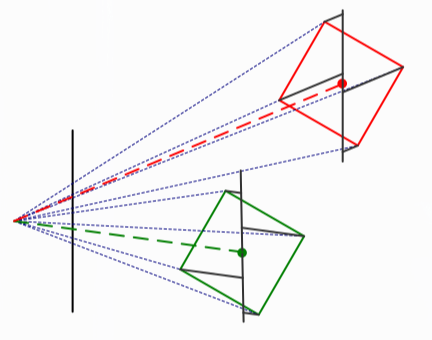
\includegraphics[width=0.5\textwidth]{../_files/_images/para-perspective.png}
    \caption{A para-perspective projection. Note how a 3D object is projected onto the intermediate plane: projection lines are parallel to the projection line of the object center.}
    \label{fig:para-perspective-projection}
\end{figure}

Para-perspective is an affine projection:
$$\tilde{\mathbf{x}}=\begin{bmatrix}
a_{11} & a_{12} & a_{13} & a_{14} \\
a_{21} & a_{22} & a_{23} & a_{24} \\
0 & 0 & 0 & 1
\end{bmatrix}\tilde{\mathbf{p}}.$$

\subsection{Projective}
For a 3D point in inhomogeneous coordinates, the projective model divides its $x$ and $y$ coordinates by $z$, finally dropping the $z$ coordinate:
$$\mathbf{x}=\begin{bmatrix}
p_{x}/p_{z} \\
p_{y}/p_{z} \\
1
\end{bmatrix}.$$
While, when considering homogeneous coordinates, as we have seen in the previous section, this becomes linear:
$$\tilde{\mathbf{x}}=\begin{bmatrix}
1 & 0 & 0 & 0 \\
0 & 1 & 0 & 0 \\
0 & 0 & 1 & 0
\end{bmatrix}\tilde{\mathbf{p}}.$$
When applying this 3D to 2D transformation, we lose the $w$ coordinate of $\tilde{\mathbf{p}}$, which encodes the universal scale and so the distance of the 3D point from the camera.
We will see that a more clever transformation will keep this information.

\subsection{Camera intrinsics}
Recall that our goal is to reconstruct the 3D world starting from the camera 2D image plane.
In this section, we will see how to map 2D pixel coordinates to 3D rays with a homography.

\subsubsection{From the pixel coordinates to the camera coordinates}
Once a photograph is taken, what we have is a pixel matrix, generated by the camera sensor matrix\footnote{The sensor matrix is that physical hardware, made of light-detecting elements, that captures the image.}, where each pixel is identified by two indices $\mathbf{x}=(x_{s},y_{s})$.
We need to pass from the digital, discrete pixel coordinates to some physical, real coordinates.
To achieve this, we will scale the pixel indices by the pixel spacing (i.e. the physical distance between a light detector and the following one) so that we will obtain the physical position of the pixel on the camera sensor matrix. More precisely, these coordinates will be embedded in a 3D space to obtain the 3D coordinates of the pixel on the camera sensor matrix.

Then, we will address the rotation and translation of the sensor matrix with respect to the camera reference system (i.e., the one with the pinhole as origin and the $z$ axis as the projection line\footnote{One can see the projection line as the line that exits orthogonal from the camera lens}).
In this way, we will reconstruct the internal geometry of the camera i.e. we will know where pixels are actually located inside the camera with respect to the camera reference system.

Formally, given a pixel homogeneous coordinates $\bar{\mathbf{x}}=(x_{s},y_{s},1)$, we can discover its 3D inhomogenous coordinates inside the camera, i.e. $\mathbf{p}$, with the following transformation:
$$\mathbf{p}=\begin{bmatrix}
\mathbf{R}_{s} & \mathbf{c}_{s}
\end{bmatrix}
\begin{bmatrix}
s_{x} & 0 & 0 \\
0 & s_{y} & 0 \\
0 & 0 & 0 \\
0 & 0 & 1
\end{bmatrix}
\begin{bmatrix}
x_{s} \\
y_{s} \\
1
\end{bmatrix}
$$
The first transformation (right to left) scales the $x$ and $y$ pixel coordinates by the pixel spacings $s_x$ and $s_y$ and then embeds the homogeneous pixel inside a homogeneous\footnote{The choice of a homogeneous space for these intermediate coordinates allows to seamlessly multiply these coordinates by the rotation + translation matrix of the subsequent transformation.} 3D space. In this 3D space, pixels all lie on the image plane, which in this case is $z=0$:
$$\begin{bmatrix}
s_xx_s \\
s_yy_s \\
0 \\
1
\end{bmatrix}.$$

Next, we rotate ($\mathbf{R}_s$) the image plane with respect to the camera reference system and apply a translation ($\mathbf{c}_s$) so that the top-left point on the image plane is mapped to the position of the top-left light-detecting element $\mathbf{c}_s$.
Actually, we do this rotation + translation by multiplying the intermediate vector by the $\begin{bmatrix} \mathbf{R}_s & \mathbf{c}_s \end{bmatrix}$ matrix.
The final result is $\mathbf{p}$, which represents the 3D inhomogeneous coordinates of the point on the sensor plane with respect to the camera reference system.

From now on, we will describe this whole transformation via a single matrix:
$$\mathbf{p}=\mathbf{M}_{s}\bar{\mathbf{x}}_{s}.$$

Recall that every column of a rotation matrix is a base vector of the rotated coordinate system. This means that all $\mathbf{r}_{1},\mathbf{r}_{2},\mathbf{r}_{3}$ s.t. $\mathbf{R}=\begin{bmatrix}\mathbf{r}_{1}& \mathbf{r}_{2} & \mathbf{r}_{3}\end{bmatrix}$ are base vectors of the coordinate system encoded in $\mathbf{R}$.
However, when multiplying the two matrices, $\mathbf{r}_{3}$ gets lost and $\mathbf{r}_{1}$ and $\mathbf{r}_{2}$ get multiplied by $s_{x}$ and $s_{y}$, respectively.

We can then expand the product:
$$\mathbf{p}=\begin{bmatrix}
s_{x}\mathbf{r}_{1} & s_{y}\mathbf{r}_{2} & \mathbf{c}_{s}
\end{bmatrix}\bar{\mathbf{x}}_{s}$$
where we can note that $s_{x}\mathbf{r}_{1}$ is the unit step in the image plane along the $x_{s}$ axis, and so $s_{y}\mathbf{r}_{2}$ for the $y_{s}$ axis.

%TODO: why is M defined by 8 parameters?
$\mathbf{M}_{s}$ is defined by 8 parameters. However, since sensor spacing and its distance from the origin are entangled, we only have 7 DOF.
However, estimating this matrix is impractical, and so many prefer to estimate a $3\times 3$ homogeneous matrix, which we will discuss in a moment.

The 3D inhomogeneous point $\mathbf{p}$ belongs to a ray that starts from $\mathbf{p}_{c}$, the real point that generates the ray, passes through the camera pinhole $\mathbf{O}_{c}$ and intercepts the image plane in $\mathbf{p}$.
Since $\mathbf{p}$ and $\mathbf{p}_{c}$ belong to the same ray, they are related by an unknown scaling:
$$\mathbf{p}_{c}=\alpha\mathbf{p}.$$
Hence, we can express the relation between $\mathbf{p}_{c}$ and $\tilde{\mathbf{x}}_{s}$ with the following transformation:
$$\tilde{\mathbf{x}}_{s}=\mathbf{M}_{s}^{-1}\mathbf{p}= \beta \mathbf{M}^{-1}_{s}\mathbf{p}_{c}=\mathbf{K}\mathbf{p}_{c}$$
where $\mathbf{K}\in 3\times3$ is called the \keyword{calibration matrix} and describes the camera intrinsics.

\subsubsection{Camera intrinsics and extrinsics}
\keyword{Intrinsics} describe how the pixels generated by the sensor matrix are positioned in space with respect to the camera reference system, while \keyword{extrinsics} describe the position of the whole camera in space with respect to the world reference system.
So, if you pick up a camera and move it around a room, its extrinsics change constantly, but its intrinsics remain completely unchanged. You can modify intrinsics by performing a zoom, which physically moves the pinhole away from the image plane.

%TODO: follow up: why is K defined by 7 parameters?
We have already discussed that $\mathbf{K}$ should have 7 DOF in theory, but has 8 DOF in practice. However, $\mathbf{K}$ is usually treated as an upper-triangular matrix with $5$ DOF, since we cannot recover the full $\mathbf{K}$ matrix based on external measurement alone.

\subsubsection{From camera coordinates to real world coordinates}
For a 3D point $\mathbf{p}_{c}$, to really know its actual position in space $\mathbf{p}_{w}$ (subscript $c$ stands for \emph{camera}, while $w$ stands for \emph{world}), we need to apply a rotation and translation to our camera reference system. This means that the full mapping from the world points to the image pixels is
$$\tilde{\mathbf{x}}_{s}=\mathbf{P}\mathbf{p}_{w} = \mathbf{K} [\mathbf{R} \mid \mathbf{t}]\mathbf{p}_{w}=\mathbf{K}\mathbf{p}_{c}$$
where $[\mathbf{R}\mid \mathbf{t}]$ describes the camera extrinsics and $\mathbf{P}$ is called the \keyword{camera matrix}.

\begin{figure}[h]
    \centering
    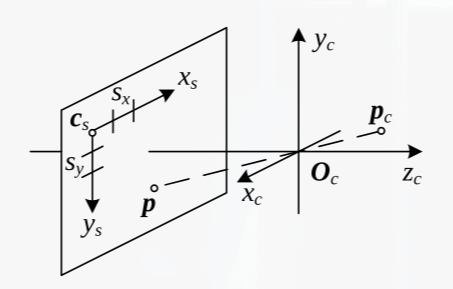
\includegraphics[width=0.5\textwidth]{../_files/_images/from-pixels-to-camera-points.png}
    \caption{This image shows how a camera-centered point $\mathbf{p}_c$ (i.e. a real word point $\mathbf{p}_w$ that is mapped to the camera reference system) generates a ray that intercepts the image plane in $\mathbf{p}$.}
    \label{fig:from-pixels-to-camera-points}
\end{figure}

Suppose we pick any arbitrary 3D rotation matrix $\mathbf{R}_1$. Because rotation matrices are orthogonal, we have $\mathbf{R}_1 \mathbf{R}_1^{\top} = \mathbf{I}$.
Now, let's modify our intrinsics and extrinsics by inserting $\mathbf{R}_1$:
\begin{enumerate}
\item Post-multiply $\mathbf{K}$ by $\mathbf{R}_1$:
$$\mathbf{K}' = \mathbf{K} \mathbf{R}_1$$
\item Pre-multiply $[\mathbf{R} \mid \mathbf{t}]$ by $\mathbf{R}_1^{\top}$:
$$[\mathbf{R} \mid \mathbf{t}]' = \mathbf{R}_1^{\top} [\mathbf{R} \mid \mathbf{t}] = [\mathbf{R}_1^{\top} \mathbf{R} \mid \mathbf{R}_1^{\top} \mathbf{t}]$$
\end{enumerate}

Now compute the new projection matrix $\mathbf{P}'$:
$$\mathbf{P}' = \mathbf{K}' [\mathbf{R} \mid \mathbf{t}]' = (\mathbf{K} \mathbf{R}_1) (\mathbf{R}_1^{\top} [\mathbf{R} \mid \mathbf{t}])$$
Using matrix associativity:
$$\mathbf{P}' = \mathbf{K} (\mathbf{R}_1 \mathbf{R}_1^{\top}) [\mathbf{R} \mid \mathbf{t}] = \mathbf{K} \mathbf{I} [\mathbf{R} \mid \mathbf{t}] = \mathbf{K} [\mathbf{R} \mid \mathbf{t}] = \mathbf{P}$$
Since we have made no assumptions on $\mathbf{R}_{1}$, we conclude that there are infinite many choices of $\mathbf{K}$ and $[\mathbf{R}\mid \mathbf{t}]$ to obtain the same $\mathbf{P}$.
In other words, we can rotate the sensor matrix (intrinsics) or the camera orientation in the world (extrinsics) and obtain the very same image.

Since camera calibration algorithms estimate the whole $\mathbf{P}$ matrix, we cannot derive $\mathbf{K}$ and $[\mathbf{R}\mid \mathbf{t}]$ alone. This is the \emph{intrinsic-extrinsic ambiguity}. Nonetheless, researchers have conventionally derived $\mathbf{K}$ using QR factorization. This is why $\mathbf{K}$ is usually represented as a upper-triangular matrix.

\begin{observation}{QR decomposition}
QR factorization (or QR decomposition) is a linear algebra method that decomposes any real $m \times n$ matrix $\mathbf{A}$ into the product of two distinct matrices:
$$\mathbf{A} = \mathbf{Q}\mathbf{R}$$
\begin{itemize}
\item $\mathbf{Q}$ (Orthogonal Matrix): An $m \times m$ matrix whose columns are orthonormal (mutually perpendicular unit vectors), satisfying $\mathbf{Q}^{\top} \mathbf{Q} = \mathbf{I}$. Geometrically, $\mathbf{Q}$ represents pure rotations and reflections without changing lengths.
\item $\mathbf{R}$ (Upper-Triangular Matrix): An $m \times n$ matrix where all entries below the main diagonal are zero ($r_{ij} = 0$ for $i > j$).
\end{itemize}

In this context, $\mathbf{R}$ is not a rotation matrix.
\end{observation}

Upon calibration, $\mathbf{K}$ can have several standard forms. The most general one is
$$\mathbf{K}=\begin{bmatrix}
f_{x} & s & c_{x} \\
0 & f_{y} & c_{y} \\
0 & 0 & 1
\end{bmatrix}$$
where:
\begin{itemize}
\item $f_{x}=fm_{x}$ and $f_{y}=fm_{y}$ are the focal lengths considering $m_{x}$ and $m_{y}$ as unit length respectively. Focal length is the distance between the optical center (lens center) and the image plane. These two lenghts are different when pixels are not perfectly square, i.e. if $m_{x}\neq m_{y}$;
\item $s$ encodes any possible skew i.e. when the $x$ and $y$ axes are not perfectly orthogonal;
\item $(c_{x}, c_{y})$ is the image center (also called principal point) in pixel coordinates.
\end{itemize}

For recent cameras, we usually have $s=0$ and $f_{x}=f_{y}=f$, and so the standard form of $\mathbf{K}$ is:
$$\mathbf{K}=\begin{bmatrix}
f & 0 & c_{x} \\
0 & f & c_{y} \\
0 & 0 & 1
\end{bmatrix}.$$

Focal length is expressed depending on the units used to measure pixels. So, if pixel coordinates use integer values, focal length can be expressed in pixel values.

\subsubsection{Preserving depth}
Sometimes, it is preferable for $\mathbf{P}$ to have full rank, i.e. to be a $4\times4$ matrix. For this to happen, we add a row to $[\mathbf{R} \mid \mathbf{t}]$ and a row and a column to $\mathbf{K}$:
$$\tilde{\mathbf{P}}=\begin{bmatrix}
\mathbf{K} & \mathbf{0} \\
\mathbf{0}^{\top} & 1
\end{bmatrix}
\begin{bmatrix}
\mathbf{R} & \mathbf{t} \\
\mathbf{0}^{\top} & 1
\end{bmatrix}=\tilde{\mathbf{K}}\mathbf{E}$$
where $\tilde{\mathbf{K}}$ is the full-rank calibration matrix and $\mathbf{E}$ is a 3D rigid body transformation matrix in homogeneous coordinates obtained by adding a row to the rotation + translation $\mathbf{R}$ matrix.

As before, this matrix maps real world 3D points to pixel coordinates, but, in this case, in homogeneous coordinates.

By keeping the fourth row to construct a full-rank $4 \times 4$ matrix $\tilde{\mathbf{P}}$, we can backproject $\tilde{\mathbf{x}}_{s}$ to $\mathbf{p}_{w}$ using the inverse $\tilde{\mathbf{P}}^{-1}$.

Let's expand the $\tilde{\mathbf{P}} \bar{\mathbf{p}}_w$ product:
$$\tilde{\mathbf{P}} \bar{\mathbf{p}}_w = \tilde{\mathbf{K}}\bar{\mathbf{p}}_{c} = \begin{bmatrix} f_x & s & c_x & 0 \\ 0 & f_y & c_y & 0 \\ 0 & 0 & 1 & 0 \\ 0 & 0 & 0 & 1 \end{bmatrix} \begin{bmatrix} x_c \\ y_c \\ z_c \\ 1 \end{bmatrix} = \begin{bmatrix} f_x x_c + s y_c + c_x z_c \\ f_y y_c + c_y z_c \\ z_c \\ 1 \end{bmatrix}$$

In pinhole perspective projection, 2D screen coordinates are formed by dividing physical camera coordinates $(x_c, y_c)$ by the optical depth $z_c$ (distance along the camera projection line).

To perform perspective division by depth, the entire vector must be divided by its depth $z_{c}$:
$$\begin{bmatrix} \frac{f_x x_c + s y_c + c_x z_c}{z_c} \\ \frac{f_y y_c + c_y z_c}{z_c} \\ \frac{z_c}{z_c} \\ \frac{1}{z_c} \end{bmatrix} = \begin{bmatrix} x_s \\ y_s \\ 1 \\ d \end{bmatrix}=\begin{bmatrix}
\bar{\mathbf{x}}_{s} \\
d
\end{bmatrix}$$
where $d=\frac{1}{z_{c}}$ is called \keyword{disparity}.

In this way, the 3D to 2D projection $\tilde{\mathbf{P}}$ has preserved the depth information, which would be lost with the non full-rank projection matrix $\mathbf{P}$.

Note that we can extend $\mathbf{P}$ with the row that best fits our needs and not necessarily with the previously considered one. In fact, by remapping the last row as $s_{3}\begin{bmatrix}\hat{\mathbf{n}}_{0} & c_{0}\end{bmatrix}$ and performing the matrix multiplication, to which follows the division by $z$, we obtain
$$d = \frac{s_3}{z} (\hat{\mathbf{n}}_0 \cdot \mathbf{p}_w + c_0)$$
, which is called projective depth or \keyword{parallax}, as the fourth component. 

Let $\hat{\mathbf{n}}_{0}$ be the normal vector of the plane $\mathcal{P}$ (called the \keyword{reference plane}) described by the equation:
$$\mathbf{x}^{\top}\hat{\mathbf{n}} + c = 0$$
and let $\| \hat{\mathbf{n}}_{0} \|=1$.

Let $\mathbf{x}_0$ be a fixed point that lies on $\mathcal{P}$. Because $\mathbf{x}_0 \in \mathcal{P}$, it satisfies the plane equation:
$$\mathbf{x}_0^{\top}\hat{\mathbf{n}} + c = 0 \implies c = -\mathbf{x}_0^{\top}\hat{\mathbf{n}}$$
Let $\mathbf{x}$ be an arbitrary point in space. The displacement vector pointing from the reference point on the plane $\mathbf{x}_0$ to $\mathbf{x}$ is $(\mathbf{x} - \mathbf{x}_0)$.

The orthogonal (shortest) signed distance $d$ from $\mathbf{x}$ to the plane is obtained by projecting the vector $(\mathbf{x} - \mathbf{x}_0)$ onto the unit normal vector $\hat{\mathbf{n}}$:
$$d = (\mathbf{x} - \mathbf{x}_0) \cdot \hat{\mathbf{n}} = (\mathbf{x} - \mathbf{x}_0)^{\top}\hat{\mathbf{n}}$$
Expanding the vector product:
$$d = \mathbf{x}^{\top}\hat{\mathbf{n}} - \mathbf{x}_0^{\top}\hat{\mathbf{n}}$$
Substituting the identity $c = -\mathbf{x}_0^{\top}\hat{\mathbf{n}}$ yields:
$$d = \mathbf{x}^{\top}\hat{\mathbf{n}} + c$$
The absolute Euclidean distance $D$ is the magnitude of this result: $D = \vert{}\mathbf{x}^{\top}\hat{\mathbf{n}} + c\vert{}$.

Now, let's consider this geometrically. In the following figure, we have drawn the plane $\mathcal{P}$ with equation $x=1$, that has $\hat{n}=(1,0,0)$ as unit normal vector (drawn in blue). Consider $A \equiv (1,1,1) \in \mathcal{P}$ and another point $B\equiv (3,2,3)\not\in \mathcal{P}$. We can see that the projection (drawn in red) of the displacement vector (drawn in green) onto $\hat{n}$ equals (in length) the projection of $B$ onto $\mathcal{P}$.

\begin{figure}[h]
    \centering
    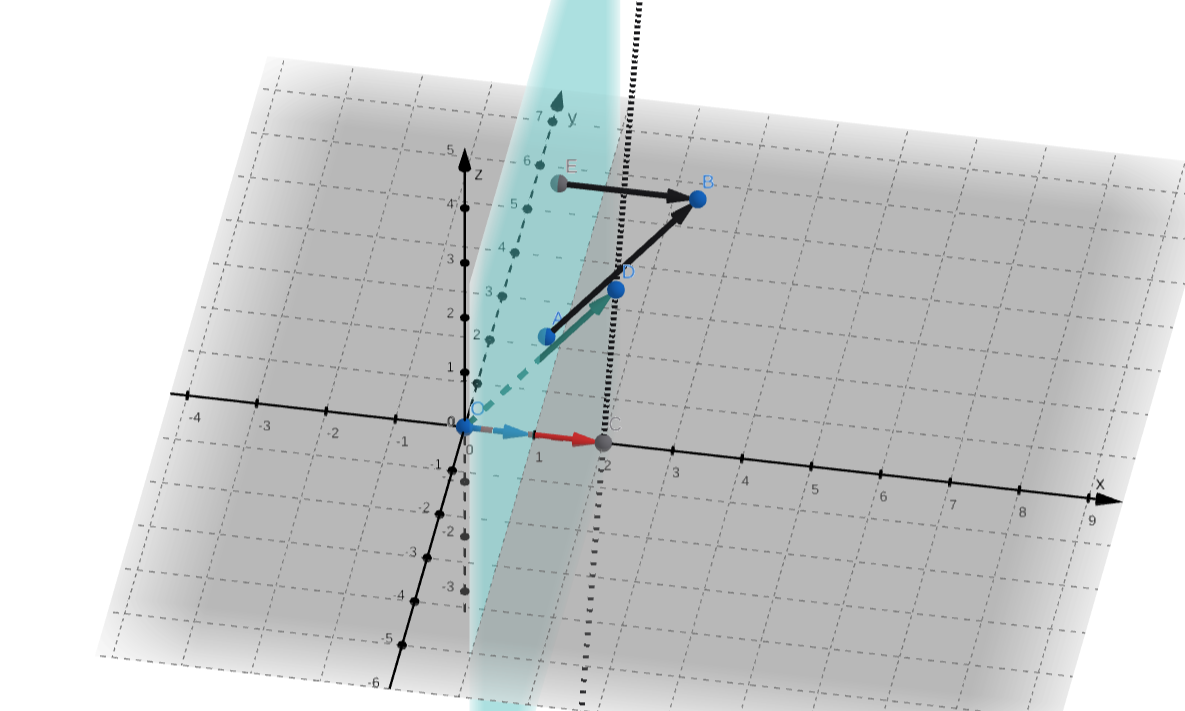
\includegraphics[width=0.5\textwidth]{../_files/_images/reference-plane-1.png}
    \label{fig:reference-plane-1}
\end{figure}

It is clearer from a point of view that is perpendicular to the $x$ and $y$ axes, as in the following figure.

\begin{figure}[h]
    \centering
    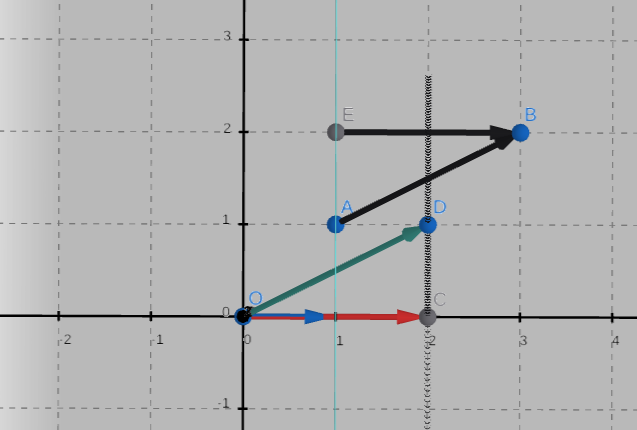
\includegraphics[width=0.5\textwidth]{../_files/_images/reference-plane-2.png}
    \label{fig:reference-plane-2}
\end{figure}

If $\hat{\mathbf{n}}$ is not unitary ($\Vert{}\hat{\mathbf{n}}\Vert{} \neq 1$), the expression yields a scaled signed distance equal to $\Vert{}\hat{\mathbf{n}}\Vert{} \cdot d$.

Choosing $\hat{\mathbf{n}}=0$ and $c_{0}=1$ (and $s_{3}=1$) causes the parallax to become the standard disparity:
$$d = \frac{s_3}{z} (\hat{\mathbf{n}}_0 \cdot \mathbf{p}_w + c_0) \implies d = \frac{1}{z} (\mathbf{0} \cdot \mathbf{p}_w + 1) = \frac{1}{z}$$
Geometrically, this means putting the reference plane at infinity. In fact, in $\mathcal{P}^3$ (as we have seen when discussing primitives) the plane at infinity is described by
$$[\hat{\mathbf{n}}\mid 1]=(0,0,0,1)$$

\subsubsection{Mapping from one camera to another}
Intuitively, we could reconstruct the depth of a 3D point by taking pictures of it from different points of view, just like we do with our two eyes.

Using the full rank camera matrix $\tilde{\mathbf{P}}=\tilde{\mathbf{K}}\mathbf{E}$, we know that the following transformation leads from the 3D point to its related pixel on the image plane:
$$\tilde{\mathbf{x}}_{0}=\tilde{\mathbf{P}}_{0}\mathbf{p}_{w}=\tilde{\mathbf{K}}_{0}\mathbf{E}_{0}\mathbf{p}_{w}$$
where the subscript $0$ means that this pixel was obtained by the camera with index $0$.
Analogously, we can capture the same point with camera $1$:
$$\tilde{\mathbf{x}}_{1}=\tilde{\mathbf{P}}_{1}\mathbf{p}_{w}=\tilde{\mathbf{K}}_{1}\mathbf{E}_{1}\mathbf{p}_{w}$$
We could reconstruct $\mathbf{p}_{w}$ with
$$\mathbf{p}_{w}=\tilde{\mathbf{P}}_{0}^{-1}\tilde{\mathbf{x}}_{0}.$$
Then, we can project this reconstructed point to the image plane of camera $1$:
$$\tilde{\mathbf{x}}_{1}=\tilde{\mathbf{P}}_{1}\tilde{\mathbf{P}}^{-1}_{0}\tilde{\mathbf{x}}_{0}=\mathbf{M}_{10}\tilde{\mathbf{x}}_{0}.$$
Unfortunately, we do not usually have access to the depth information of pixels of a standard image. However, let's assume the 3D scene is planar (i.e., it lies entirely on a plane) and that we have built the last row of $\tilde{\mathbf{P}}$ to encode the reference plane and that the 3D scene lies exactly on the reference plane.

In this scenario, every pixel $\tilde{\mathbf{x}}$ will have null parallax and so we can ignore the last row of $\tilde{\mathbf{{P}}}$. At this point, we can also ignore the last column of $\mathbf{M}$:
$$\mathbf{M}_{10}\tilde{\mathbf{x}}_{0}=
\begin{bmatrix}
m_{11} & m_{12} & m_{13} & m_{14} \\
m_{21} & m_{22} & m_{23} & m_{24} \\
m_{31} & m_{32} & m_{33} & m_{34} \\
m_{41} & m_{42} & m_{43} & m_{44} \\
\end{bmatrix}
\begin{bmatrix}
\tilde{x}_{1} \\
\tilde{x}_{2} \\
\tilde{x}_{3} \\
0
\end{bmatrix}=
\tilde{x}_{1}\begin{bmatrix}
m_{11} \\
m_{21} \\
m_{31} \\
m_{41}
\end{bmatrix}
+
\tilde{x}_{2}\begin{bmatrix}
m_{12} \\
m_{22} \\
m_{32} \\
m_{42}
\end{bmatrix}
+
\tilde{x}_{3}\begin{bmatrix}
m_{13} \\
m_{23} \\
m_{33} \\
m_{43}
\end{bmatrix}
+
0\begin{bmatrix}
m_{14} \\
m_{24} \\
m_{34} \\
m_{44}
\end{bmatrix}
$$
as well as the last row of $\mathbf{M}$ since we don't need to store the parallax coordinate. So, the equation reduces to:
$$\tilde{\mathbf{x}}_{1}=\tilde{\mathbf{H}}_{10}\tilde{\mathbf{x}}_{0}$$
where $\tilde{\mathbf{x}}_{0},\tilde{\mathbf{x}}_{1}$ are $3$-vectors (homogeneous 2D vectors) and $\tilde{\mathbf{H}}_{10}$ is a $3\times 3$ matrix.

Another case where we can easily link pixels between two cameras is when camera $0$ and camera $1$ differ from a simple rotation. In this case, we have $\mathbf{P}=\mathbf{K}\mathbf{R}$ instead of $\mathbf{P}=\mathbf{K}[\mathbf{R}|\mathbf{t}]$ and so:
$$\tilde{\mathbf{x}}_{1}=\mathbf{P}_{1}\mathbf{P}^{-1}_{0}\tilde{\mathbf{x}}_{0}=\mathbf{K}_{1}\mathbf{R}_{1}\mathbf{R}^{-1}_{0}\mathbf{K}_{0}^{-1}\tilde{\mathbf{x}}_{0}=\mathbf{K}_{1}\mathbf{R}_{10}\mathbf{K}_{0}^{-1}\tilde{\mathbf{x}}_{0}$$
with all matrices being $3\times 3$ and $\mathbf{R}_{10}$ being the rotation from the camera $0$ position to the camera $1$ position.

\subsection{Zoom vs. distance ambiguity}
First, we assume the simplified calibration matrix $\mathbf{K}$
$$\mathbf{K} = \begin{bmatrix} f & 0 & c_x \\ 0 & f & c_y \\ 0 & 0 & 1 \end{bmatrix}$$
Applying the camera's rigid extrinsics $(\mathbf{R}, \mathbf{t})$ transforms a 3D point $\mathbf{p}$ into camera-centered coordinates $\mathbf{p}_c$:
$$\mathbf{p}_c = \mathbf{R}\mathbf{p} + \mathbf{t} = \begin{bmatrix} \mathbf{r}_x \cdot \mathbf{p} + t_x \\ \mathbf{r}_y \cdot \mathbf{p} + t_y \\ \mathbf{r}_z \cdot \mathbf{p} + t_z \end{bmatrix} = \begin{bmatrix} x_c \\ y_c \\ z_c \end{bmatrix}$$
where $\mathbf{r}_x, \mathbf{r}_y, \mathbf{r}_z$ are the three rows of the rotation matrix $\mathbf{R}$, and $t_x, t_y, t_z$ are the components of the translation vector $\mathbf{t}$.

Multiplying $\mathbf{p}_c$ by the intrinsic matrix $\mathbf{K}$ gives the homogeneous pixel vector $\tilde{\mathbf{x}}_s$:
$$\tilde{\mathbf{x}}_s = \mathbf{K} \mathbf{p}_c = \begin{bmatrix} f & 0 & c_x \\ 0 & f & c_y \\ 0 & 0 & 1 \end{bmatrix} \begin{bmatrix} x_c \\ y_c \\ z_c \end{bmatrix} = \begin{bmatrix} f x_c + c_x z_c \\ f y_c + c_y z_c \\ z_c \end{bmatrix}$$

To convert from homogeneous coordinates to actual 2D pixel coordinates $(x_s, y_s)$, we must divide the coordinates by $z_{c}$:
$$x_s = \frac{f x_c + c_x z_c}{z_c} = f \frac{x_c}{z_c} + c_x = f \frac{\mathbf{r}_x \cdot \mathbf{p} + t_x}{\mathbf{r}_z \cdot \mathbf{p} + t_z} + c_x$$
$$y_s = \frac{f y_c + c_y z_c}{z_c} = f \frac{y_c}{z_c} + c_y = f \frac{\mathbf{r}_y \cdot \mathbf{p} + t_y}{\mathbf{r}_z \cdot \mathbf{p} + t_z} + c_y$$
We can now note that for $t_{z} \gg \| \mathbf{p} \|$, the coordinate depends on the $f / t_{z}$ ratio, i.e. the ratio of the focal length to the point's distance from the camera. Intuitively, when we keep this ratio fixed, the image scale remains the same.

For this reason, we can define a scale parameter $s=f / t_{z}$ and an inverse distance parameter $\eta_{z} = 1 / t_{z}$ s.t. the equations become
$$x_s = s \frac{\mathbf{r}_x \cdot \mathbf{p} + t_x}{\eta_{z}\mathbf{r}_z \cdot \mathbf{p} + 1} + c_x$$
$$y_s = s \frac{\mathbf{r}_y \cdot \mathbf{p} + t_y}{\eta_{z}\mathbf{r}_z \cdot \mathbf{p} + 1} + c_y$$
In this way, we have obtained two separated parameters: $s$ and $\eta_{z}$. In fact, the first directly measures the 2D size of the object on the image plane, while the second can be estimated by measuring the \keyword{foreshortening} as an object rotates.

\begin{observation}{Foreshortening}
    Imagine holding your hand up and pointing your index finger directly at your eyes.
    You see the tip of your finger, while its actual length disappears into the depth of your vision. 
    If you turn your hand $90^\circ$ so your finger is parallel to your face, you see its full length.
    Foreshortening is the difference between these two views: the steeper the angle relative to your line of sight, the more compressed the object appears in 2D.

    You can repeat this experiment by moving your finger at different distances from your eyes and see that the same angle of rotation yields different lenghts.
\end{observation}

Moreover, by adopting $\eta_{z}$ and $s$, we can cover both projective and orthographic models. In fact, for $t_{z}$ big, we have $\eta_{z}=0$ and so the previous equations become:
$$x_s = s(\mathbf{r}_x \cdot \mathbf{p} + t_x) + c_x$$
$$y_s = s(\mathbf{r}_y \cdot \mathbf{p} + t_y) + c_y$$
which completely ignore depth.

